\chapter{Introduction}
\label{sec:introduction}
In the past decade, multi-copter type drones have been developed and spread all around the world for applications ranging from geographical mapping to entertainment. Furthermore, the latest developments on Miniature Aerial Vehicles (MAVs) have involved more physical interactions with the environment, power optimization and more Degrees of Freedom (DoFs) which leads to significantly more complex control pipelines. For instance, the Omnidirectional Miniature Aerial Vehicle (OMAV) at the Autonomous Systems Lab (ASL) in ETH Zurich and outlined in \cite{Bodie_Proceeding_2020} consists of 6 pairs of co-axially aligned propellers with tilting axis. Mentioned platform is depicted in Figure \ref{fig: mav_photo}.
\begin{figure}
    \centering
    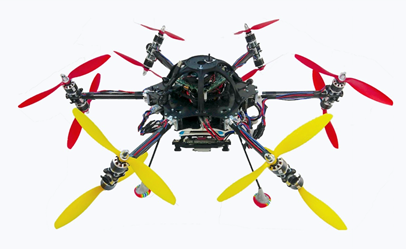
\includegraphics{images/mav_photo.png}
    \caption{ASL OMAV}
    \label{fig: mav_photo}
\end{figure}

Although this novel setup is highly versatile, the current rotor speed control implementation is open-loop, assuming relatively accurate and linear throttle to actual rotor speed mapping. Furthermore, the high number of propellers increases the chance of an individual failure on flight, requiring status information to be sent towards the flight controller (FC). Another important consideration is the aerodynamic interference between coaxial propellers, which surely causes disturbances leading to slower tracking. The extend of this disturbances is still unknown. Therefore, \cite{Bodie_pre_release_2020} recommends to perform a more thorough identification of this OMAV dynamics to decrease disturbances during optimal control design.

\textit{Objectives} In this context, this report will describe my work during my semester project with the following objectives:
\begin{itemize}
    \item Familiarize with current firmware available for FC-ESC communication.
    \item Achieve rotor speed feedback from the ESC to the FC.
    \item Explore different ESC typologies and 
    \item Investigate the characteristics of driving the Brush-less Direct Current (BLDC) motors using an ESC.
    \item Investigate features available in modern ESCs.
\end{itemize}